\documentclass[12pt,a4paper]{article}
\usepackage[latin1]{inputenc}
\usepackage{amsmath}
\usepackage{amsfonts}
\usepackage{amssymb}
\usepackage{graphicx}
\author{Carter Rhea}
\title{Homework 2}
\begin{document}
	\maketitle
\section{Problem 1}
	$$\sigma,_x + f =0 $$
	$$u = g \ at \ x=0 $$
	$$\sigma = h \ at \ x = L$$

	Weak form:
	$$\int_0^L w*(\sigma,_x + f)dx = 0 $$
	By applying the divergence theorem we obtain,
	$$-\int w,_x\sigma dx + (w\sigma)\biggl|_0^L + \int_0^L wfdx = 0$$
	Now applying the boundary conditions and noting the $\forall w \in V \ w(0)=0$ yields,
	$$\int_0^Lw,_x\sigma dx = \int_0^L wfdx + w(L)h $$
	As usual, let us discretize:
	$$u^h = sum_{A=2}^{n_{el}+1} N_A(x)d_A+gN_1(x) $$
	$$w^h = sum_{A=2}^{n_{el}+1} N_A(x)c_A $$
	Plugging into the weak form gives us,
	$$\int_0^Lw^h,_x\hat{\sigma}(u^h,_x)dx = \int_0^L w^hf dx + w^h(L)h $$
	Hence,
	$$F^{int} =  \int_0^Lw^h,_x\hat{\sigma}(sum_{B=1}^{n_{el}+1} N_B,_x(x)d_B)dx$$
	$$F^{ext} = \int_0^L N_A(x)f dx + N_A(x)(L)h  $$
	Note that $A=2,...n_{en}+1$ and $d_i$ is such that $d_1 = g$.
	
	As for the tangent stiffness matrix:
	\begin{align*}
	K^e_{ab} &= \frac{\partial f^{int \ e}}{\partial d_b^e} \\
	&= \frac{\partial}{\partial d_b^e} \Big[ \int_{x_1}^{x_2} N_a,_x(x) \hat{\sigma} \big(\sum_{c=1}^{N_{en}}N_c,_xd_c^e\big)dx \Big] \\
	&= \int_{x_1^e}^{x_2^e}N_a,_x\frac{\partial \hat{\sigma}}{\partial \epsilon}\big(\sum_{c=1}^{N_{en}}N_c,_xd_c^e\big) \frac{\partial }{\partial d_b^e}\big(\sum_{c=1}^{N_{en}}N_c,_xd_c^e\big) d_b^e dx\\
	&= \int_{x_1^2}^{x_2^e}N_a,_xE(\epsilon\biggl|_{d=d^{e }} )N_b,_x dx\\		
	\end{align*}
	
	Although it at first appears that the consistent tangent is symmetric, we actually are unable to claim such due to the nonlinearity of $E$.
	
	\section{Problem 2}
	
\begin{figure}[h!]
	\centering
	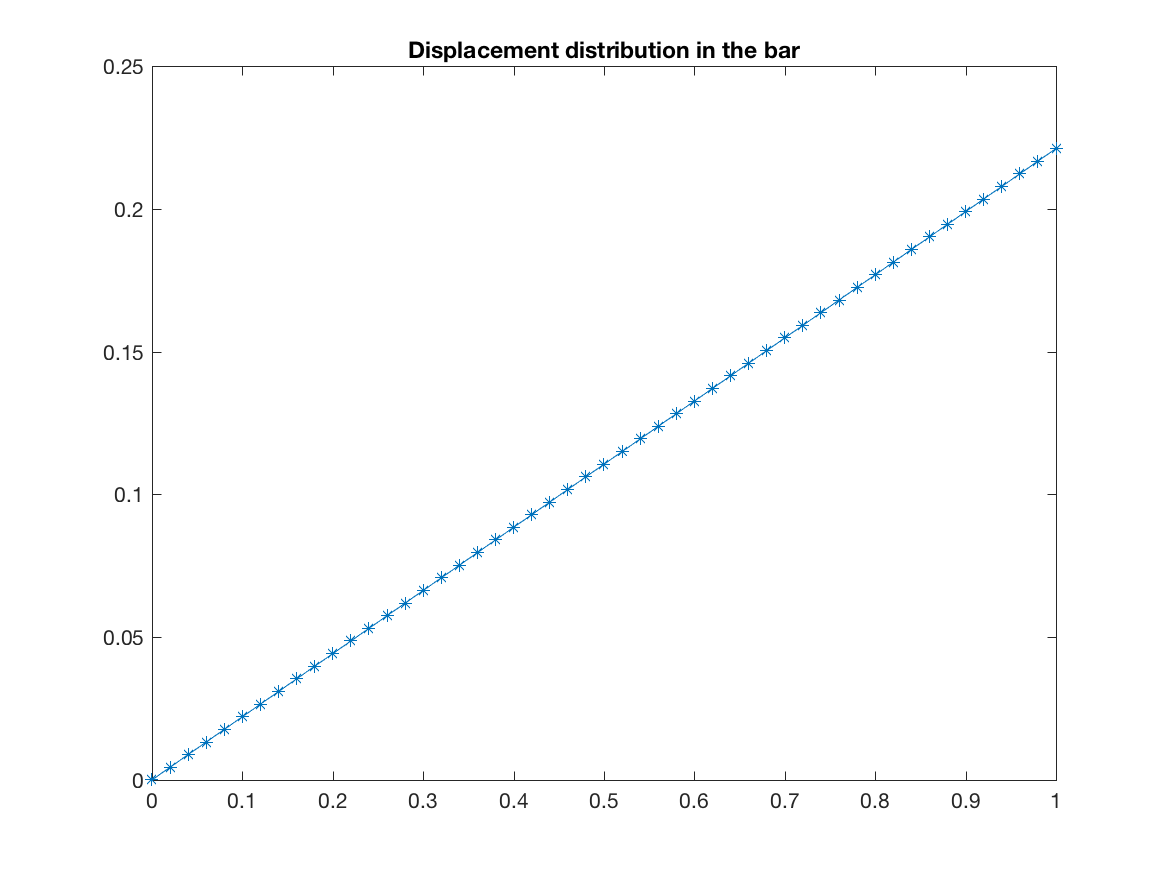
\includegraphics[width=0.7\linewidth]{problem2}
	\caption{final solution with 100 loading steps}
	\label{fig:problem2}
\end{figure}
	
	\section{Problem 3}
	Show (using Taylor's theorem) that Newton-Raphson itertaion converges and that the order of convergence is 2.\\
	\textbf{Solution}:
	Let $R$ be the residual.\\
	By Taylor's theorem truncated at the second derivative we have,
	$$0=R+R'\Delta d + \frac{R''}{2} \Delta d^2 $$
	subtracting both sides by $R$ and dividing by $R'^{-1}$ yields,
	$$R'^{-1}R = \Delta d + R'^{-1}R''\frac{\Delta d}{2} $$
	Further isolating 	$\Delta d$ and noting that it is equal to $d-d^i$ we have,
	$$(d^i-R'^{-1}R)-d = R'^{-1}R''\frac{(d^i-d)^2}{2} $$
	Note that $d^i-R'^{-1}R = d^{i+1}$ and $d^i-d = e_i$. Hence we arrive at the following:
	$$e_{i+1} = e_{i}^2\frac{R'^{-1}R''}{2} $$
	We are given that $\frac{R'^{-1}R''}{2} \leq c$ hence we have the following quadratic convergence:
	
	$$\frac{e_{i+1}}{e_{i}^2} < c $$
	\newpage
	\section{Problem 4}
	
	
	
\begin{figure}[h!]
	\centering
	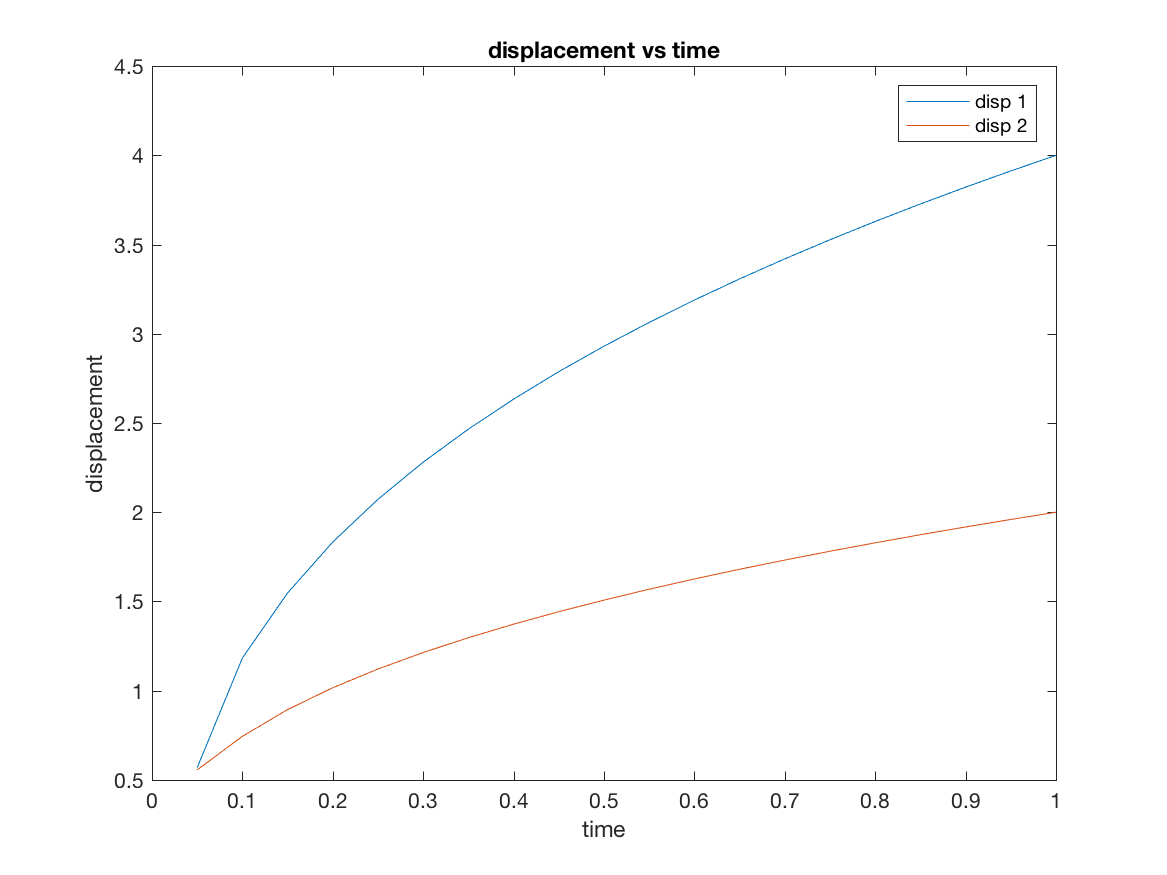
\includegraphics[width=0.7\linewidth]{problem4}

	\label{fig:problem4}
\end{figure}
	
	
\end{document}